\documentclass[a4paper,14pt]{extreport}
	\usepackage[left=1.5cm,right=1.5cm,
	    top=1.5cm,bottom=2cm,bindingoffset=0cm]{geometry}
	\usepackage{scrextend}
	\usepackage[T1,T2A]{fontenc}
	\usepackage[utf8]{inputenc}
	\usepackage[english,russian,ukrainian]{babel}
	\usepackage{tabularx}
	\linespread{1.5}
	\usepackage{amssymb}
	\usepackage{fp}
	\usepackage{color}
	\usepackage{amsmath}
	\usepackage{mathrsfs}
	\usepackage{listings}
	\usepackage{graphicx}
	\graphicspath{ {./images/} }
	\usepackage{lipsum}
	\usepackage{xcolor}
	\usepackage{multirow}
	%\usepackage[table,xcdraw]{xcolor}
	\usepackage{hyperref}
	\usepackage{tcolorbox}
	\usepackage{tikz}
	\usepackage[framemethod=TikZ]{mdframed}
	\usepackage{wrapfig,boxedminipage,lipsum}
	\mdfdefinestyle{MyFrame}{%
	linecolor=blue,outerlinewidth=2pt,roundcorner=20pt,innertopmargin=\baselineskip,innerbottommargin=\baselineskip,innerrightmargin=20pt,innerleftmargin=20pt,backgroundcolor=gray!50!white}
	 \usepackage{csvsimple}
	 \usepackage{supertabular}
	\usepackage{pdflscape}
	\usepackage{fancyvrb}
	%\usepackage{comment}
	\definecolor{ggreen}{rgb}{0.4,1,0}
	\definecolor{rred}{rgb}{1,0.1,0.1}
	\definecolor{aquamarine}{rgb}{0.5, 1.0, 0.83}
	\definecolor{amber}{rgb}{1.0, 0.75, 0.0}
	\definecolor{babyblue}{rgb}{0.54, 0.81, 0.94}
	\definecolor{buff}{rgb}{0.94, 0.86, 0.51}
	\definecolor{internationalorange}{rgb}{1.0, 0.31, 0.0}
	\definecolor{lightmauve}{rgb}{0.86, 0.82, 1.0}
	\definecolor{mediumaquamarine}{rgb}{0.4, 0.8, 0.67}
	\usepackage{array,tabularx}
	\usepackage{colortbl}
	
	\usepackage{varwidth}
	\tcbuselibrary{skins}
	\usepackage{fancybox}

	\usetikzlibrary{calc}
	\makeatletter
	\newlength{\mylength}
	\xdef\CircleFactor{1.1}
	\setlength\mylength{\dimexpr\f@size pt}
	\newsavebox{\mybox}
	\newcommand*\circled[2][draw=blue]{\savebox\mybox{\vbox{\vphantom{WL1/}#1}}\setlength\mylength{\dimexpr\CircleFactor\dimexpr\ht\mybox+\dp\mybox\relax\relax}\tikzset{mystyle/.style={circle,#1,minimum height={\mylength}}}
	\tikz[baseline=(char.base)]
	\node[mystyle] (char) {#2};}
	\makeatother
	\usepackage{pgfplots}
    \pgfplotsset{compat=1.9}


	\usepackage{float}
	\usepackage{wrapfig}
	\usepackage{framed}
	%for nice Code{
	\lstdefinestyle{customc}{
	  belowcaptionskip=1\baselineskip,
	  breaklines=true,
	  frame=L,
	  xleftmargin=\parindent,
	  language=C,
	  showstringspaces=false,
	  basicstyle=\small\ttfamily,
	  keywordstyle=\bfseries\color{green!40!black},
	  commentstyle=\itshape\color{purple!40!black},
	  identifierstyle=\color{blue},
	  stringstyle=\color{orange},
	}
	\lstset{escapechar=@,style=customc}
	\usepackage{enumitem}
%}


\begin{document}
\newtcbox{\xmybox}[1][red]{on line, arc=7pt,colback=#1!10!white,colframe=#1!50!black, before upper={\rule[-3pt]{0pt}{10pt}},boxrule=1pt, boxsep=0pt,left=6pt,right=6pt,top=2pt,bottom=2pt}
\pagecolor{white}
\begin{titlepage}
	\begin{center}
	\large
	Національний технічний університет України \\ "Київський політехнічний інститут імені Ігоря Сікорського"


	Факультет Електроніки

	Кафедра мікроелектроніки
	\vfill

	\textsc{ЗВІТ}\\

	{\Large Про виконання РГР\\
	з дисципліни: «Вакуумна та плазмова електроніка»\\[1cm]

	


	}
	\bigskip
	\end{center}
	\vfill

	\newlength{\ML}
	\settowidth{\ML}{«\underline{\hspace{0.4cm}}» \underline{\hspace{2cm}}}
	\hfill
	\begin{minipage}{1\textwidth}
	Виконавець:\\
	Студент 3-го курсу \hspace{4cm} $\underset{\text{(підпис)}}{\underline{\hspace{0.2\textwidth}}}$  \hspace{1cm}Б.\,П.~Фіцай\\


	Перевірив: \hspace{5.9cm} $\underset{\text{(підпис)}}{\underline{\hspace{0.2\textwidth}}}$  \hspace{1cm}О.\,М.~Бевза\\

	\end{minipage}

	\vfill

	\begin{center}
	2021
	\end{center}
\end{titlepage}

\begin{center}\textbf{\fbox{Завдання}}\end{center}\par
	\begin{enumerate}
		\item 	Дивимось на графіки побудовані для п.3 лабораторної роботи.
		\begin{enumerate}[label=1.\arabic*]
			\item Визначити частоту червоної границі фотоефекту.
			\item Необхідно визначити напругу запирання для кожного елементу при інтенсивності 50 \% та 100\%.  Пояснити, чому напруги запирання відрізняються при різній інтенсивності.
			\item  Побудувати графіки залежностей напруги запирання від частоти ( у вас вказані довжини хвиль, отже їх треба перерахувати в частоту) для випадку інтенсивності 50\% та 100\%.  Для кожного матеріалу (у кожного свої три матеріала).
			\item Визначити з цих нових побудованих графіків роботу виходу в точці (будь-якій, назвіть її А) за вашим власним вибором, яка розташована десь посередині отриманого графіку. Для всіх трьох матеріалів. Для обох значень інтенсивності (50\% та 100\%). Порівняйте отримані значення роботи виходу при двох різних інтенсивностей для кожного матеріалу та зробити висновки.
			\item  Розрахувати кінетичну швидкість електронів для точки А для всіх трьох матеріалів.
			\item  Порівняти отримане із розрахунку значення роботи виходу з відомими значеннями роботи виходу (довідкові дані, вказати джерело) та розрахувати абсолютну та відносну помилки. Зробити для трьох ваших матеріалів матеріалів.
			\item  Отримані результати звести до таблиці, де повинен бути вказаний кожен з трьох матеріалів та розраховані для нього значення: частота червоної границі фотоефекту, напруга запирання (для двох інтенсивностей), робота виходу в точці А (дві інтенсивності), кінетична швидкість електронів в точці А (для двох інтенсивностей 50\% та 100\%).
			\item Зробіть перевірку правильності виконання розрахунків за формулою Ейнштейна для фотоефекту.
		\end{enumerate}

		\item Беремо  графіки зроблені до пункту 4, де було побудовано залежності струму від інтенсивності. Ви вибирали самі три довжини хвилі. У кожного вибрано свій один матеріал. Робимо:
		\begin{enumerate}[label=2.\arabic*]
			\item Побудуйте ваш графік в інших координатах, де вісь х- довжина хвилі, вісь у-струм. Беремо значення струму для Інтенсивності 50\%.
			\item Побудуйте самі (ваші припущення) на вашому новому графіку іншим кольором як буде виглядати ця залежність, якщо інтенсивність буде складати, а далі за списком вибираємо свій варіант.
		\end{enumerate}
		\item Пояснити чому струм змінився саме так. Дивимось на графіки побудовані для пункта 5. Де залежності енергії від частоти. Треба:
		\begin{enumerate}[label=3.\arabic*]
			\item Визначити яка саме енергія стоїть у вас по осі ігрек. Це повна енергія фотону чи робота виходу чи кінетична енергія електрона чи щось інше? Відповідь аргументовано пояснити.
		\end{enumerate}
\end{enumerate}
\newpage
%\begin{center}\textbf{\fbox{Виконання роботи}}\end{center}\par
	
%-----------------------------------------1.1
\textbf{Завдання 1}
	\begin{table}[h!]
		\begin{center}
			\caption{Визначення частоти червоної межі фотоефекту}
			\begin{tabular}{|c|c|}
			\hline
			Речовина & Частота червоної границі фотоефекту, $10^{15}$ Гц \\ \hline
			Na                & 0,5                        \\ \hline
			Ca                & 0,8                          \\ \hline
			Cu                & 1,2                        \\ \hline
			\end{tabular}
			\label{tab2}
		\end{center}
	\end{table}

	
%-----------------------------------------1.2-1.3

	За наступною формулою знайду  частоту:
	\begin{equation}{}
		 v = \dfrac{c}{\lambda}
		\label{eq1}
	\end{equation}
	\begin{table}[h]
		\begin{center}
			\begin{tabular}{|c|c|}
			\hline
			$\lambda$, нм & $f$ $10^{15}$ Гц \\ \hline
			200               & 1,5                   \\ \hline
			400               & 0,7                  \\ \hline
			440               & 0,6                  \\ \hline
			470               & 0,6                  \\ \hline
			\end{tabular}
		\end{center}
	\end{table}
	
			
	

	

	
			
		
	\begin{center}
	
	\begin{table}[h]
		\begin{center}
		\begin{tabular}{|c|c|c|}
			\hline
			\multicolumn{3}{|c|}{Na} \\ \hline
			 & \multicolumn{2}{c|}{$U_{\text{з}}$, B} \\ \cline{2-3} 
			\multirow{-2}{*}{$f\cdot 10^{15}$, Гц} & 50\% & 100\% \\ \hline
			0.63 & 0 & 0 \\ \hline
			0.68 & 0 & 0 \\ \hline
			0.7 & -1.7 & -1.7 \\ \hline
			1.5 & -5.9 & -6 \\ \hline
		\end{tabular}
		\end{center}
	\end{table}
	\begin{tikzpicture}%Na
		\begin{axis}[table/col sep = semicolon,
		title={Na},
		xlabel = {$f\cdot 10^{15},\text{ Гц}$},
		ylabel = {$U_{\text{з}}, B$},
		height = 0.25\paperheight, 
		width =  0.25\paperwidth,
		%legend pos = north west,
		ymajorgrids=true,
		xmajorgrids=true,
		grid style=dashed,
		legend style={nodes={scale=0.7, transform shape}}]
		\legend{ 
		\text{50\%}, \text{100\%}};
		\addplot table [x={b},y={c}]{1.2-1.3.csv};
		\addplot table [x={b},y={d}]{1.2-1.3.csv};
		\end{axis}
	\end{tikzpicture}	
	
	\begin{table}[!h]
		\begin{center}
		\begin{tabular}{|c|c|c|}
			\hline
			\multicolumn{3}{|c|}{Ca} \\ \hline
			\multirow{2}{*}{$f\cdot 10^{15}$, Гц} & \multicolumn{2}{c|}{$U_{\text{з}}$, B} \\ \cline{2-3} 
			 & 50\% & 100\% \\ \hline
			0.63 & 0 & 0 \\ \hline
			0.68 & 0 & 0 \\ \hline
			0.7 & 0 & 0 \\ \hline
			1.5 & -3 & -3.8 \\ \hline
		\end{tabular}
		\end{center}
	\end{table}
	\begin{tikzpicture}
		\begin{axis}[table/col sep = semicolon,
		title={Ca},
		xlabel = {$f\cdot 10^{15},\text{ Гц}$},
		ylabel = {$U_{\text{з}}, B$},
		height =  0.25\paperheight, 
		width =  0.25\paperwidth,
		ymajorgrids=true,
		xmajorgrids=true,
		grid style=dashed,
		legend style={nodes={scale=0.7, transform shape}}]
		\legend{ 
		\text{50\%}, \text{100\%}};
		\addplot table [grid style = both, x={g},y={h}]{1.2-1.3.csv};
		\addplot table [grid style = both, x={g},y={i}]{1.2-1.3.csv};
		\end{axis}
	\end{tikzpicture}
	
	\begin{table}[!h]
		\begin{center}
		\begin{tabular}{|c|c|c|}
			\hline
			\multicolumn{3}{|c|}{Cu} \\ \hline
			\multirow{2}{*}{$f\cdot 10^{15}$, Гц} & \multicolumn{2}{c|}{$U_{\text{з}}$, B} \\ \cline{2-3} 
			 & 50\% & 100\% \\ \hline
			0.63 & 0 & 0 \\ \hline
			0.68 & 0 & 0 \\ \hline
			0.7 & -3.3 & -3.4 \\ \hline
			1.5 & -4.2 & -4.3 \\ \hline
		\end{tabular}
		\end{center}
	\end{table}
	\begin{tikzpicture}%Cu
		\begin{axis}[table/col sep = semicolon,
			title={Cu},
			xlabel = {$f\cdot 10^{15},\text{ Гц}$},
			ylabel = {$U_{\text{з}}, B$},
			height = 0.25\paperheight, 
			width = 0.25\paperwidth,
			ymajorgrids=true,
			xmajorgrids=true,
    		grid style=dashed,
    		legend style={nodes={scale=0.7, transform shape}}]
			\legend{ 
			\text{50\%}, \text{100\%}};
			\addplot table [grid style = both, x={l},y={m}]{1.2-1.3.csv};
			\addplot table [grid style = both, x={l},y={n}]{1.2-1.3.csv};
		\end{axis}
	\end{tikzpicture}%Cu
	
	\end{center}



%-----------------------------------------1.4
	
		Роботу виходу можна знайти зa формулою: 
	\begin{equation}
		A = h\cdot f
	\end{equation}

	\FPeval\na{round( 4.14*0.9  :3)}
	\FPeval\naa{round( 4.14*0.89 :3)}

	\FPeval\ca{round( 4.14*1.05 :3)}
	\FPeval\caa{round( 4.14*1.0  :3)}

	\FPeval\cu{round( 4.14*0.7  :3)}
	


	\begin{align*}
		A_{Na-50\%} &= \na \text{ eB} \hspace{1cm} A_{Na-100\%} = \naa \text{ eB}\\
		A_{Ca-50\%} &= \ca \text{ eB}\hspace{1cm}A_{Ca-100\%} = \caa \text{ eB}\\
		A_{Cu} &= \cu \text{ eB}\\
	\end{align*}
%-----------------------------------------1.5
 

	Тепер рахуємо кінетичну швидкість електронів для точки А для всіх трьох матеріалів:
	\begin{equation}
		v = \sqrt{ \dfrac{2\cdot e\cdot U_{\text{з}}}{m} }
	\end{equation}



	Для Na
		$$v  \approx 9.9\cdot 10^{5} \text{ }\dfrac{\text{м}}{\text{c}} \hspace{1cm}v \approx 9.9 \cdot 10^{5}  \text{ }\dfrac{\text{м}}{\text{c}}$$
	

	Для Ca
		$$v\approx6.7 \cdot 10^{5}  \text{ }\dfrac{\text{м}}{\text{c}} \hspace{1cm} v\approx 7 \cdot 10^{5}  \text{ }\dfrac{\text{м}}{\text{c}}$$
	

	Для Cu
		$$v =  10.7\cdot 10^{5} \text{ }\dfrac{\text{м}}{\text{c}} $$
	
%-----------------------------------------1.6
	


\begin{table}[h]
	\begin{center}
		\begin{small}
			\begin{tabular}{|l|c|c|c|c|c|c|}
			\hline
			\multirow{3}{*}{} & \multicolumn{2}{c|}{Na} & \multicolumn{2}{c|}{Ca} & \multicolumn{2}{c|}{Cu} \\ \cline{2-7} 
			 & \multicolumn{6}{c|}{A, eB} \\ \cline{2-7} 
			 & розраховане & табличне & розраховане & табличне & розразоване & табличне \\ \hline
			\multicolumn{1}{|c|}{50\%} & 3.7 & \multirow{2}{*}{2.2} & 4.3 & \multirow{2}{*}{4} & 2.9 & \multirow{2}{*}{4.4} \\ \cline{1-2} \cline{4-4} \cline{6-6}
			\multicolumn{1}{|c|}{100\%} & 3.6 &  & 4.1 &  & 2.9 &  \\ \hline
			\end{tabular}
		\end{small}
	\end{center}
\end{table}

	Для Na 50\% похибка становить: $\triangle = 1.5$; $\delta = 68\%$\\
	Для Na 100\% похибка становить: $\triangle = 1.4$; $\delta = 63\%$\\

	Для Ca 50\% похибка становить: $\triangle = 0.3$; $\delta = 7,5\%$\\
	Для Ca 50\% похибка становить: $\triangle = 0.1$; $\delta = 2,5\%$\\

	Для Cu 50\% похибка становить: $\triangle = 1.5$; $\delta = 33\%$\\
	Для Cu 100\% похибка становить: $\triangle = 1.5$; $\delta = 33\%$\\
	
%-----------------------------------------1.7
	
	\begin{table}[h]
	\begin{small}
		\begin{tabular}{|c|c|c|c|c|c|c|}
\hline
\multicolumn{1}{|l|}{\multirow{3}{*}{}} & \multicolumn{2}{c|}{Na} & \multicolumn{2}{c|}{Ca} & \multicolumn{2}{c|}{Cu} \\ \cline{2-7} 
\multicolumn{1}{|l|}{} & \multicolumn{6}{c|}{A, eB} \\ \cline{2-7} 
\multicolumn{1}{|l|}{} & розраховане & з довідника & розраховане & з довідника & розразоване & з довідника \\ \hline
50\% & 3.1 & \multirow{2}{*}{2.2} & \multirow{2}{*}{4.4} & \multirow{2}{*}{4} & 4.5 & \multirow{2}{*}{4.4} \\ \cline{1-2} \cline{6-6}
100\% & 2.8 &  &  &  & 4.1 &  \\ \hline
\multicolumn{1}{|l|}{} & \multicolumn{6}{c|}{$U_{\text{з}}$,  В} \\ \hline
50\% & \multicolumn{2}{c|}{-2.8} & \multicolumn{2}{c|}{-1.3} & \multicolumn{2}{c|}{-3.4} \\ \hline
100\% & \multicolumn{2}{c|}{-2.9} & \multicolumn{2}{c|}{-1.4} & \multicolumn{2}{c|}{-3.4} \\ \hline
\multicolumn{1}{|l|}{} & \multicolumn{6}{c|}{V,  $\cdot 10^{5}  \text{ }\dfrac{\text{м}}{\text{c}}$} \\ \hline
50\% & \multicolumn{2}{c|}{9.9} & \multicolumn{2}{c|}{6.7} & \multicolumn{2}{c|}{10.7} \\ \hline
100\% & \multicolumn{2}{c|}{9.9} & \multicolumn{2}{c|}{7} & \multicolumn{2}{c|}{9.18} \\ \hline
\end{tabular}	
		\end{small}
	\end{table}
	Частота червоної границі фотоефекту для Na: $ 0,5 \cdot 10^{15} $ Гц\\
	Частота червоної границі фотоефекту для Ca: $ 0,8 \cdot 10^{15} $ Гц\\
	Частота червоної границі фотоефекту для Cu: $ 1,2 \cdot 10^{15} $ Гц\\
*** Дані взято з  https://himya.ru/rabota-vyxoda-elektronov.html
 
%-----------------------------------------1.8
	
	
	

%-----------------------------------------2.1 - 2.2
\textbf{Завдання 2}
	

	\begin{center}
	\begin{figure}[h!]
		\center{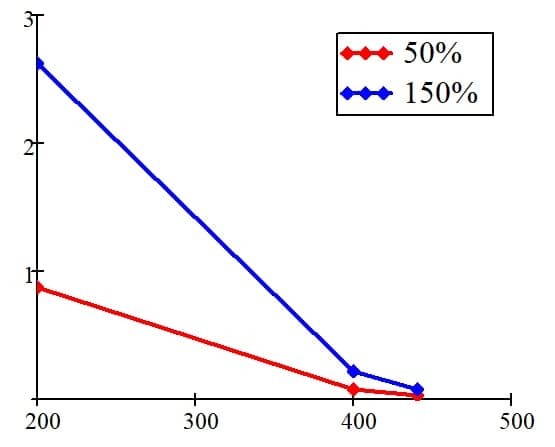
\includegraphics[width=0.4\linewidth]{2.jpg}}
		\label{ris2}
	\end{figure}
	\end{center}
	
	

%-----------------------------------------3
\textbf{Завдання 3}


	Виходячи з II законом Столетова, можна стверджувати, що на графіках з лабораторної роботи №1  по осi у в мене саме кiнетична енергiю електронiв.
















\end{document}
